%==============================================
\subsection{W--Clearance Connectivity Graph}\label{subsec:wccg}

The feasibility of routing the vehicle reduces to whether a~$W$-width corridor
connects~$\mathbf{x}_\texttt{V}^{\texttt{S}}$ and~$\mathbf{x}_\texttt{V}^{\texttt{G}}$.
A W--clearance connectivity graph (WCCG) is introduced here to encode obstacle
adjacencies under clearance~$W$ and enable fast connectivity queries.
\change{Conventional clearance checks either rasterize the workspace into an
inflated occupancy grid or query sampling-based roadmaps, and must therefore fix
a resolution and re-query the map whenever an obstacle
moves~\cite{karaman2011samplingbasedalgorithmsoptimalmotion}.
Built directly from obstacle geometry, the WCCG introduces no grid-resolution parameter in the repeated connectivity queries used during planning.}

%------------------------------
\begin{figure}[t!]
  \centering
  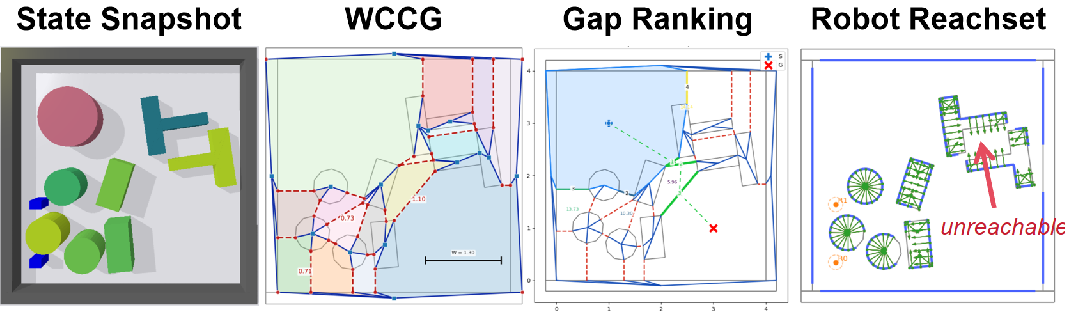
\includegraphics[width=0.9\linewidth]{figures/PIHS_top.pdf}
  \vspace{-2mm}
  \caption{\change{Core components of the physics-informed hybrid search: WCCG
  construction, gap ranking, mode generation, and physics validation.}}
  \label{fig:pihs_overview}
  \vspace{-4mm}
\end{figure}
%------------------------------

\subsubsection{Graph Construction}
The WCCG is built by decomposing all clearance-relevant obstacle and workspace
boundaries into convex components or segments.
From each component~$C$,
a centroid node~$v_c$ is created. When two components~$C_u$ and~$C_v$
have closest points~$p_u\in C_u$ and~$p_v\in C_v$ with distance less than~$W$,
bridge nodes are added at~$p_u$ and~$p_v$. These bridge nodes are
connected by a bridge--bridge edge, annotated with the gap width
$w_{uv}\triangleq\|p_u-p_v\|$, and further linked back to their centroids with
centroid--bridge edges. Narrow passages with~$w_{uv}<W$ are marked
as potential bottlenecks. The resulting graph is given by:
\begin{equation}\label{eq:wccg}
\mathcal{G}_W\triangleq(\mathcal{V},\; \mathcal{E}_c\cup\mathcal{E}_b),
\end{equation}
where~$\mathcal{V}$ are centroid and bridge nodes;
$\mathcal{E}_c$ contains centroid--bridge edges; and~$\mathcal{E}_b$ for
bridge--bridge edges with widths~$w_{uv}$.

\subsubsection{Connectivity Criterion}\label{subsubsec:bugplanner}
Once~$\mathcal{G}_W$ has been constructed, connectivity queries can be
performed without explicitly computing a geometric path. Let
$\textsf{Face}(\mathcal{G}_W)$ denote the set of connected planar faces induced
by the embedded WCCG, i.e., the maximal regions separated by obstacle
components and WCCG bottleneck edges. The criterion for~\eqref{eq:wclear}
is given by
\begin{equation}\label{eq:wccg_criterion}
\big(\mathbf{x}_\texttt{V}^{\texttt{S}},\mathbf{x}_\texttt{V}^{\texttt{G}}\in
\mathcal{F}_W(t)\big)
\wedge
\big( \exists F\in\textsf{Face}(\mathcal{G}_W):
{\mathbf{x}_\texttt{V}^{\texttt{S}},\mathbf{x}_\texttt{V}^{\texttt{G}}}\in F \big),
\end{equation}
\change{where the faces follow the standard configuration-space inflation
interpretation: expanding obstacles by a disk of radius $W/2$ turns gaps
narrower than $W$ into overlapping barriers, and non-convex obstacles are
handled through clearance-relevant decomposition, after which WCCG records the
separating bottlenecks.} The consistency between WCCG connectivity and continuous and
rasterized configuration-space references is further evaluated numerically
in Sec.~\ref{subsec:wccg-validation}.
A frontier-tracing procedure, similar to the
BugPlanner~\cite{McGuireCroonTuyls2019}, is then used to extract a skeleton
$\Sigma$ as an ordered sequence of centroid and bridge nodes. Starting from
$\mathbf{x}_\texttt{V}^{\texttt{S}}$, it casts a ray toward
$\mathbf{x}_\texttt{V}^{\texttt{G}}$ and follows the encountered frontier loop
until either a valid exit is found or a blocking cycle is returned.








%% \begin{algorithm}[t!]
%% \small
%% \caption{BugPlanner for~$W$-width connectivity (skeleton witness)}
%% \label{alg:bugplanner}
%% \DontPrintSemicolon
%% \SetKwInOut{Input}{In}\SetKwInOut{Output}{Out}
%% \Input{$\mathbf{s}^{\texttt{S}}$,~$\mathbf{s}^{\texttt{G}}$, WCCG}
%% \Output{if connected: skeleton~$\Sigma$; else: frontier loop~$\mathcal{L}$}
%%~$P\leftarrow\mathbf{s}^{\texttt{S}}$,~$\Sigma\leftarrow[\ ]$\;
%% \While{true}{
%%   \If{segment~$P\mathbf{s}^{\texttt{G}}$ hits no edge}{\Return~$\Sigma \cup \{\texttt{straight}(P,\mathbf{s}^{\texttt{G}})\}$}
%%   Build loop~$\mathcal{L}$ by angle-follow from the hit edge; append traversed edges to~$\Sigma$\;
%%   \If{$\mathrm{parity}(\mathcal{L},\,\mathbf{s}^{\texttt{S}}\mathbf{s}^{\texttt{G}})$ is odd}{\Return~$(\emptyset,\mathcal{L})$}
%%   Choose exit~$e$ on~$\mathcal{L}$ (outward normal~$\to\,\mathbf{s}^{\texttt{G}}$); append arc to~$\Sigma$;~$P\leftarrow e$ (tiny bias)\;
%% }
%% \end{algorithm}
